\documentclass{article}
\usepackage{comment}
\usepackage{float}
\usepackage{fontenc}
\usepackage{graphicx}
\usepackage{gensymb}
%\usepackage{amsfonts}
\usepackage{amssymb}
\usepackage{amsmath}
\usepackage{breqn}
\usepackage[letterpaper, margin = 0.6in]{geometry}
\usepackage{caption}
\usepackage{subcaption}
\usepackage{color}

\sloppy
\definecolor{lightgray}{gray}{0.5}
\setlength{\parindent}{0pt}
\usepackage{hyperref}

\begin{document}
\begin{center}
\textbf{\large{Project 1 - MANE 6710}} \\
\textit{Unique ID: 5284}
\end{center}
\noindent\makebox[\linewidth]{\rule{\paperwidth}{0.4pt}} 
\newline
\tableofcontents
\begin{appendix}
\listoffigures
\listoftables
\end{appendix}
\newpage
\section{Introduction}
The project in hand is to design a heat exchanger that can transfer heat from Medium 1 (water) which is at a temperature $T= 90\degree C$ to another Medium 2 (air) which is at a temperature $T= 20 \degree C$. The main motivation behind this project is to find out which design of the heat exchanger is capable of maximizing the heat flux that is transferred from one medium to another. Some of the properties of a preliminary heat exchanger and its constraints are provided: the coefficient of thermal conductivity $K = 20 \frac{W}{mK}$, Height range $h_{max}= 5cm$, $h_{min} = 1cm$ and the length of one unit of the heat exchanger $L=5cm$.
\section{Choice of Design Variables}
\begin{figure}[h]
	\centering
        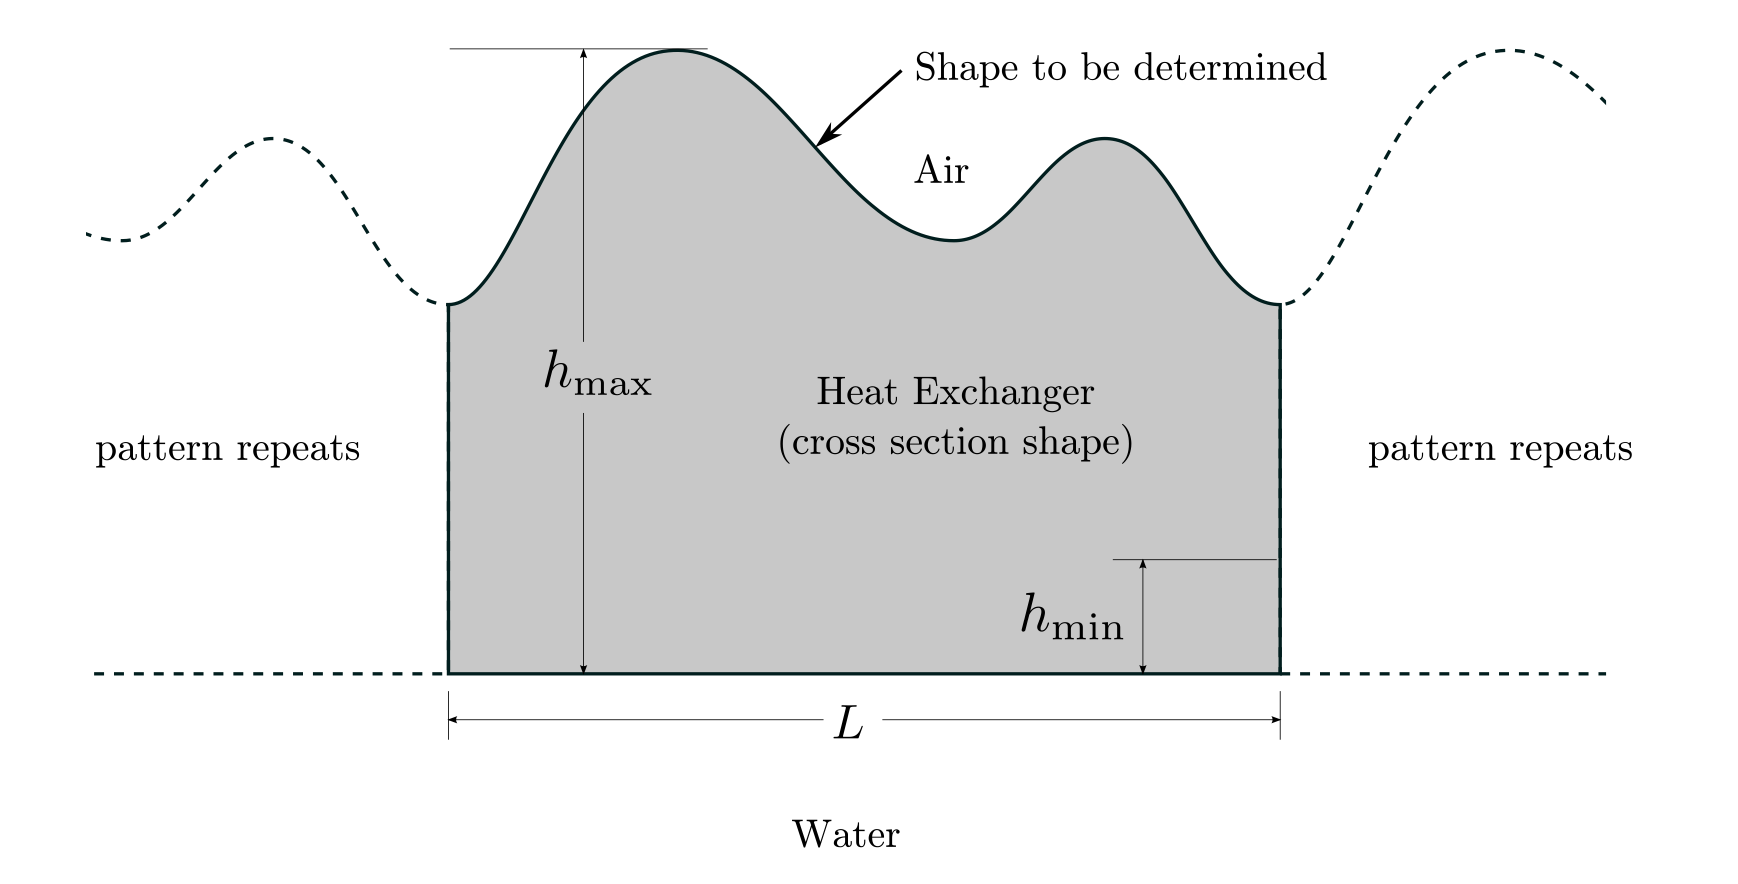
\includegraphics[width=0.5\textwidth]{Question_Image}
        	\caption{Illustration of Heat Exchanger Design Problem}
\end{figure} 
This is a 2-D cross section of the heat exchanger to be designed and it can be assumed that it extrudes into or out of the paper as a 3-D object with a width. The profile of the heat exchanger can be assumed to be a function along the X-axis which is aligned with the length $L$ of the heat exchanger: $ h(x) $.
It is mentioned in the problem statement that the this function $h(x)$ shall not be implicit. Hence we can choose to make this a function into something that can be parameterized about the values of $x$ along the length of the heat exchanger. 
The parameters $a_i$ are the design variables that can help parameterize $h(x;a)$ where $x \in \Omega$  and $ a \in \mathbb{R}^n$ 
Three different types of parameterization to proceed forward have been chosen:

\subsection{Linear Parameterization}
\begin{equation}
h(x;a) = a_1 + \sum_{j=2}^{j=n} a_j \frac{x}{L} 
\end{equation}
This parameterization is going to generate an initial profile which is linear in nature. For $a \in \mathbb{R}^n$ a linear profile looks like the example in Figure \ref{fig: linear} \\
$h(x(i)) = a_1 + \sum_{j=2}^{j=n} a_j \frac{x(i)}{L}$ as $ x $ is discretized along the length $L$ gives the height of the profile at each $x(i)$. \\
\newline
\subsection{Sinusoidal Parameterization}
\begin{equation}
h(x;a) = a_1 + \sum_{j=2}^{j=n} a_j sin\left(\frac{2\pi(j-1)x}{L}\right) 
\end{equation} 
If this parameterization is used, a sinusoidal profile is formed and an example profile for a design variable of dimension $a \in \mathbb{R}^{21}$ can be seen in Figure \ref{fig:sinusoidal}. Similar to the linear parameterization case, $x$ is discretized along the length $L$ and the above function provides the height of the profile at each $x(i)$. \\
This is linear with respect to the design variable $a$ and this profile is the linear combination of $c_ia_i$ where $c_i$ are sine waves. Or it can be thought of as superimposition of sine waves.
\subsection{Triangular Parameterization}
\begin{equation}
h(x;a) = a_1 - \frac{a_2}{\pi}\sum_{j=1}^{j=\infty} (-1)^j \frac{sin(\frac{2\pi a_3jx}{L})}{j} 
\end{equation}
A sawtooth profile that has an offset of $a_1$ is formed in this case. This parameterization requires the design variable $a \in \mathbb{R}^3$. Since it is not possible to numerically run the summation $j=1(1)n; n\rightarrow \infty$ is not possible, an appropriately large value of $n$ can be chosen. The value chosen for this project is $n = 50$. $a_2$ is the height of the sawtooth and $a_3$ is the frequency of sawtooth profile. An example profile is displayed in Figure \ref{fig:triangular}\\
One specific detail to note in the case of using a triangular parameterization is that the relationship between $h(x;a)$ and design variable $a$ is nonlinear.
\begin{figure}[h]
     \centering
     \begin{subfigure}[b]{0.4\textwidth}
         \centering
         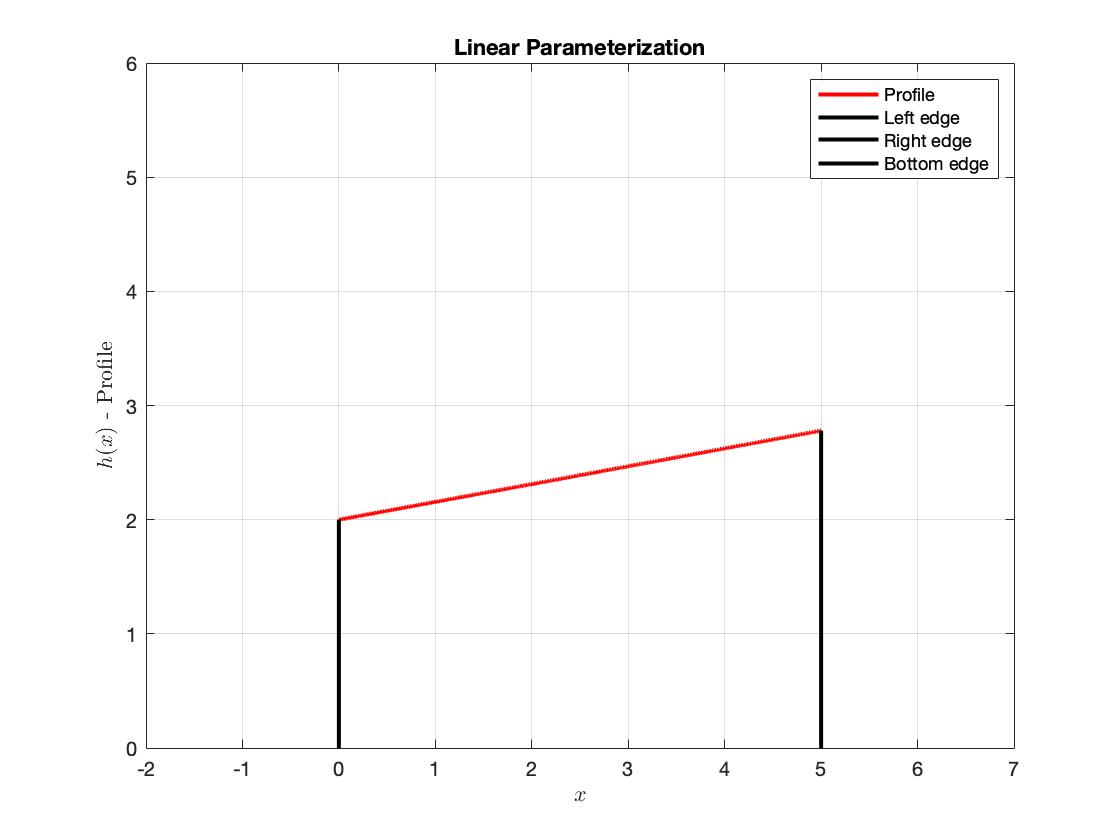
\includegraphics[width=\textwidth]{Linear_Parameterization}
         \caption{Linear Parameterization}
         \label{fig: linear}
     \end{subfigure}
     \hfill
     \begin{subfigure}[b]{0.4\textwidth}
         \centering
         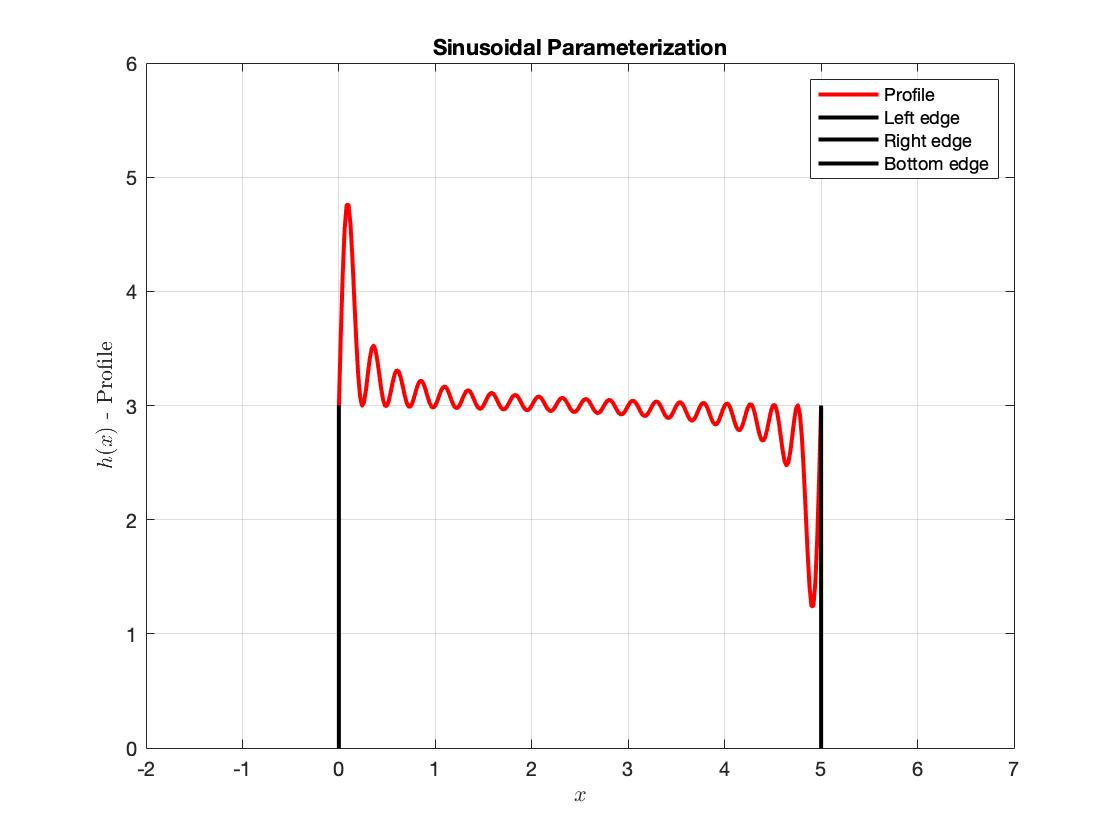
\includegraphics[width=\textwidth]{Sinusoidal_Parameterization}
         \caption{Sinusoidal Parameterization}
         \label{fig:sinusoidal}
     \end{subfigure}
     \begin{subfigure}[b]{0.4\textwidth}
         \centering
         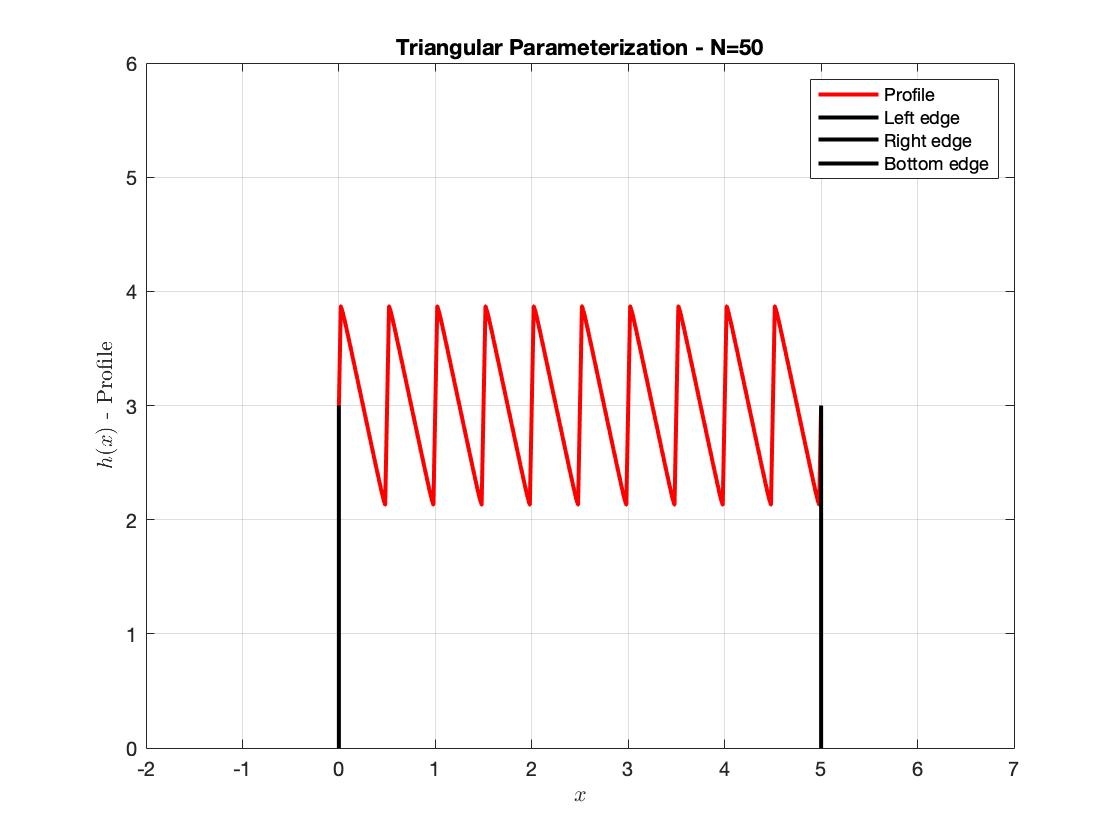
\includegraphics[width=\textwidth]{Triangular_Parameterization}
         \caption{Triangular Parameterization}
         \label{fig:triangular}
     \end{subfigure}
        \caption{Profile based on different Parameterization}
        \label{fig:three graphs}
\end{figure}
\section{Objective Function and Constraints}
The objective function is the calculation of heat flux. 
\begin{equation}
q = \int -(\kappa \nabla T )dA
\label{eqn: heat flux}
\end{equation}
This is calculated by the function \textit{\textbf{CalcFlux.m}} . This function takes in as inputs : Profile of the heat exchanger $h(x;a)$, $\kappa, L, N_x, N_y, T_{water}, T_{air}$. This function computes the steady state heat transfer using a Finite Volume approach. The geometry of this heat exchanger is made into a finite volume mesh using the function \textit{\textbf{BuildMesh.m}}. \textit{\textbf{BuildMesh.m}} requires the inputs $L, h(x;a), N_x, N_y$ and is called inside \textit{\textbf{CalcFlux.m}}. Steady state heat transfer is then solved using another function \textit{\textbf{BuildSystem.m}} which is called within \textit{\textbf{CalcFlux.m}} after building a mesh. \textit{\textbf{BuildSystem.m}} requires the inputs $L,h,N_x,N_y,\kappa, T_{water}, T_{air}$. The solver returns a Temperature field over the finite volume elements and this Temperature field can be used to calculate the heat flux using Equation.\ref{eqn: heat flux}
\section{Setting up the Optimization Problem}
The optimization problem is now set up as follows: 
\begin{equation}
\centering
\begin{split}
&\underset{a \in  \mathbb{R}^n}{max}  \; \; q(a) \\  s.t \; \; h_{min} \leq \; & h(x;a) \leq \; h_{max} 
\end{split}
\end{equation}
It is important to note that both linear and sinusoidal parameterization produces $h(x;a)$ where $a$ an $x(i)$ are linearly related each other and hence, the constraint equation can be written as $Ca \leq b$ where $C$ matrix holds the coefficients that when multiplied with the vector(design variable) $a$ produces the constraint thats always $\leq b$. However this is not the case with Triangular parameterization and a function should be specifically written in order to calculate this nonlinear inequality between $h_{min} \,\leq h(x;a) \, \leq h_{max}$. \\
The optimizer that is used in this project is an inbuilt optimization algorithm from $MATLAB$ called $fmincon(...)$. This optimizer has the function arguments: $obj, a_0, C,b,C_{eq},b_{eq}, Nonlinear \; constraints, \; Options$. $obj$ is the objective function and $a_0$ is the initial starting point\\
For the linear and sinusoidal cases, the function call to the optimizer follows $fmincon(obj, a_0, C, b, [.],[.],[.], \; Options)$ because there are no equality or nonlinear constraints involved. When triangular parameterization is used, the function call is of the form: $fmincon(obj, a_0, [.],[.],[.],[.], nonlinear\; constraint,\; Options)$. ($[.]$ means an empty matrix)\\
The code for generation of the profile $h(x;a)$, generating the objective function $q = obj(a)$ and setting up the constraints matrix $C, b$ can be found in the Appendix.
\section{Comparison of Preliminary Results}
Preliminary analysis has been done on a mesh with spacing $N_x = N_y = 100$.  
\begin{enumerate}
	\item Linear Parameterization
		\begin{itemize}
			\item Initial Condition : $a_0(1) = 2; a_0(2:21) = 0.1; \; \; \; a\in \mathbb{R}^{21}$
			\item Optimal Design Variable : \hyperlink{X_linear}{Found in Appendix}
			\item Final Top Profile: 
			\begin{figure}[H]
				\centering
				\begin{subfigure}[b]{0.45\textwidth}
         			\centering
         			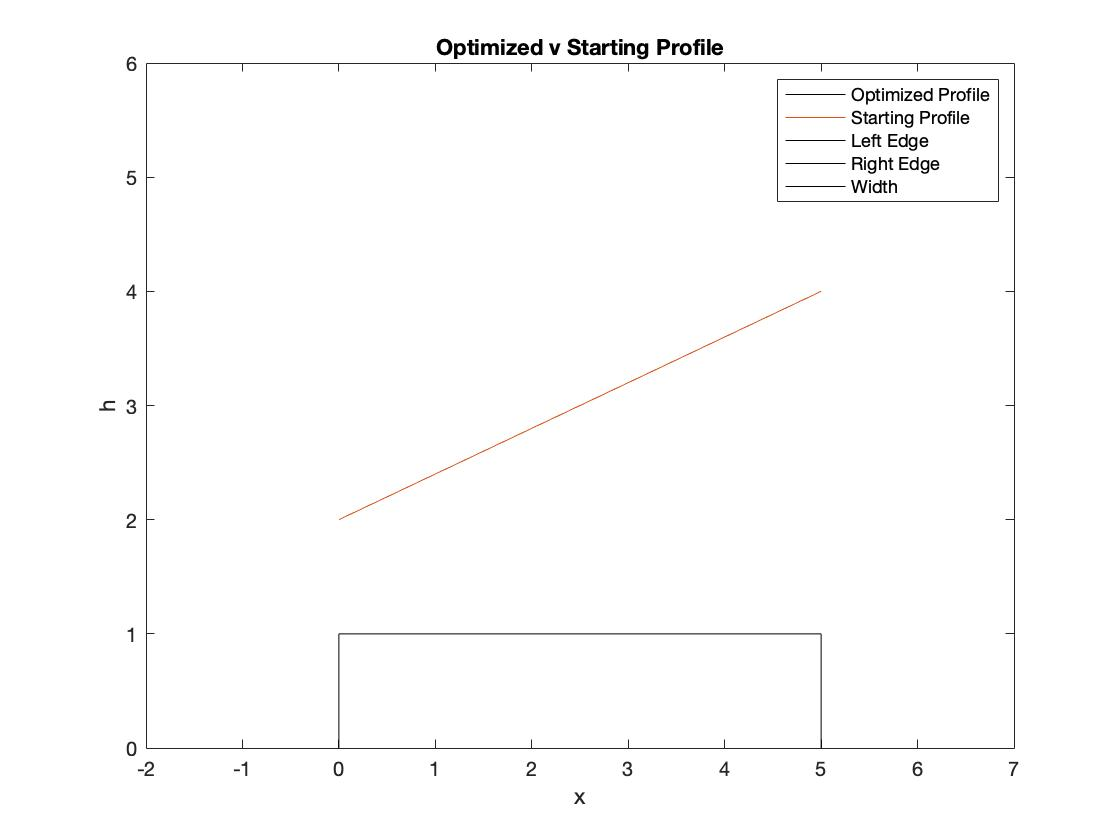
\includegraphics[width=\textwidth]{Mtd2_SP1_1}
         			\caption{Starting v Final - Linear}
         			\label{fig: linear start v end}
         		\end{subfigure}
         		\hfill
			\begin{subfigure}[b]{0.45\textwidth}
         			\centering
         			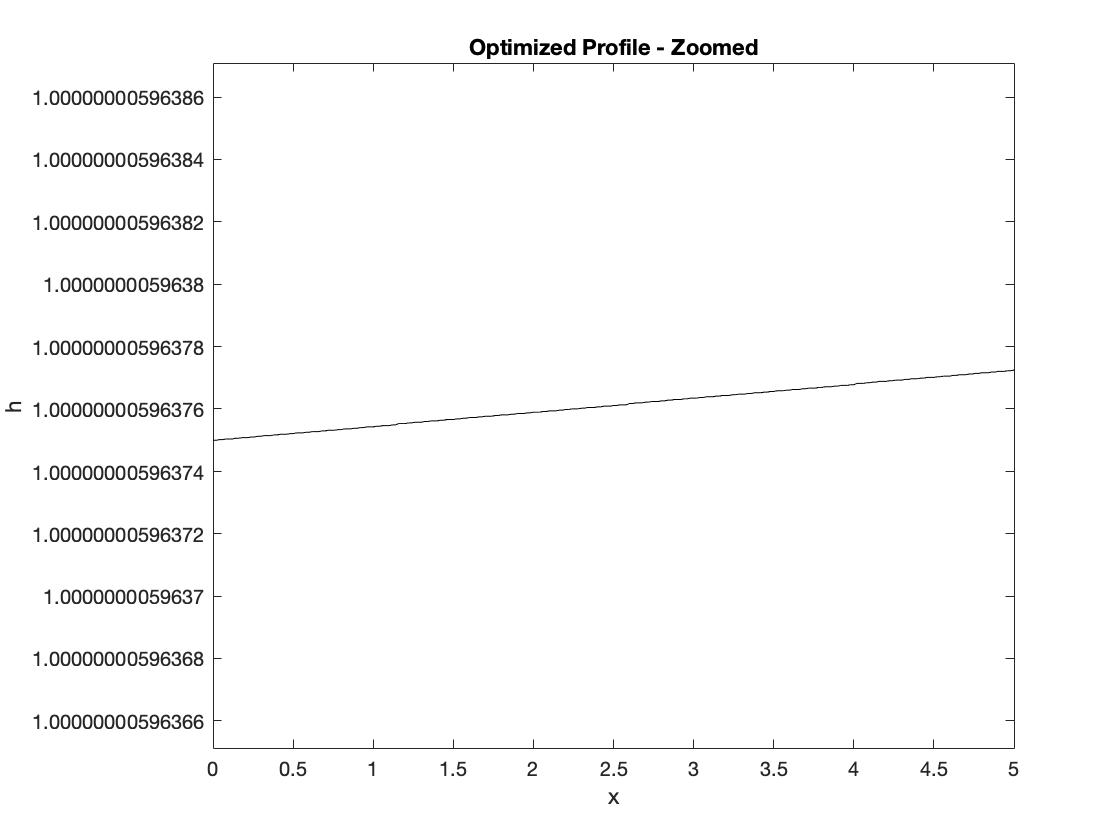
\includegraphics[width=\textwidth]{Mtd2_SP1_2}
         			\caption{Final Zoomed - Linear}
         			\label{fig: linear final zoomed}
         		\end{subfigure}
         		\caption{Optimized Profile using Linear Parameterization}
			\end{figure}
			\item Flux through Optimized profile: $6953.64 \frac{W}{m^2}$
			\item Optimizer convergence:
			\begin{enumerate}
				\item Total number of iterations: $13$
				\item The total number of function calls: $287$
				\item Algorithm used: $Interior-Point$
				\begin{figure}[H]
					\centering
					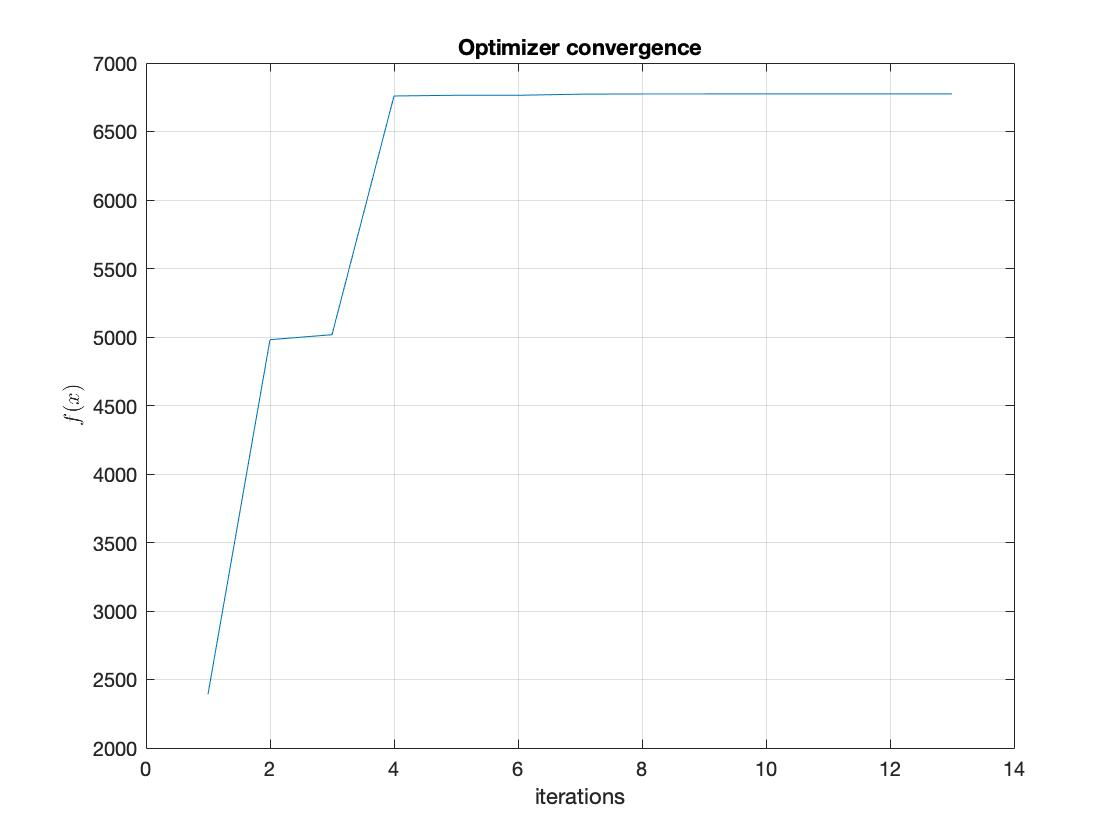
\includegraphics[width=0.5\textwidth]{Mtd2_SP1_3}
					\caption{Flux v Iterations - Linear}
					\label{fig: lin fluxIter}
				\end{figure}
			\end{enumerate}
		\end{itemize}
	\item Sinusoidal Parameterization
		\begin{itemize}
			\item Initial Condition : $a_0(1) = 3; a_0(2:21) = 0.12; \; \; \; a\in \mathbb{R}^{21}$
			\item Optimal Design Variable : \hyperlink{X-sin}{Found in Appendix}
			\item Final Top Profile: 
			\begin{figure}[H]
				\centering
				\begin{subfigure}[b]{0.45\textwidth}
         			\centering
         			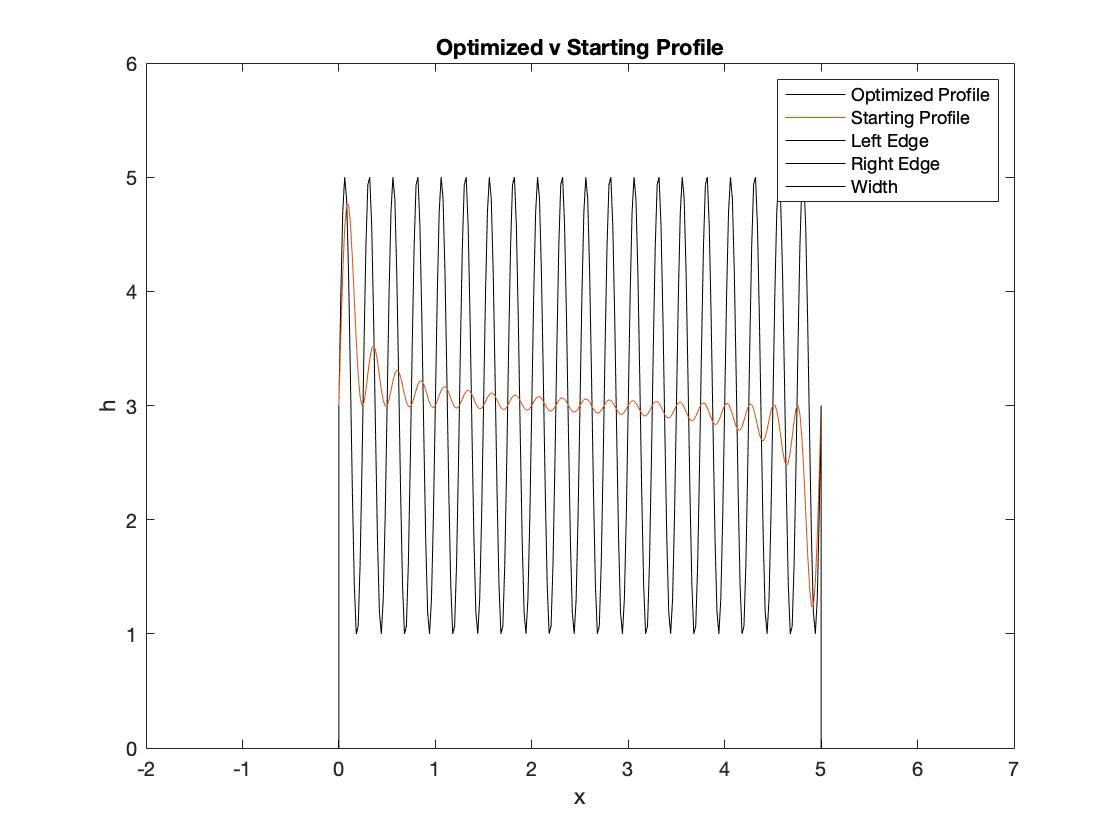
\includegraphics[width=\textwidth]{Mtd1_SP4_1}
         			\caption{Starting v Final - Sinusoidal}
         			\label{fig: sin start v end}
         		\end{subfigure}
         		\hfill
			\begin{subfigure}[b]{0.45\textwidth}
         			\centering
         			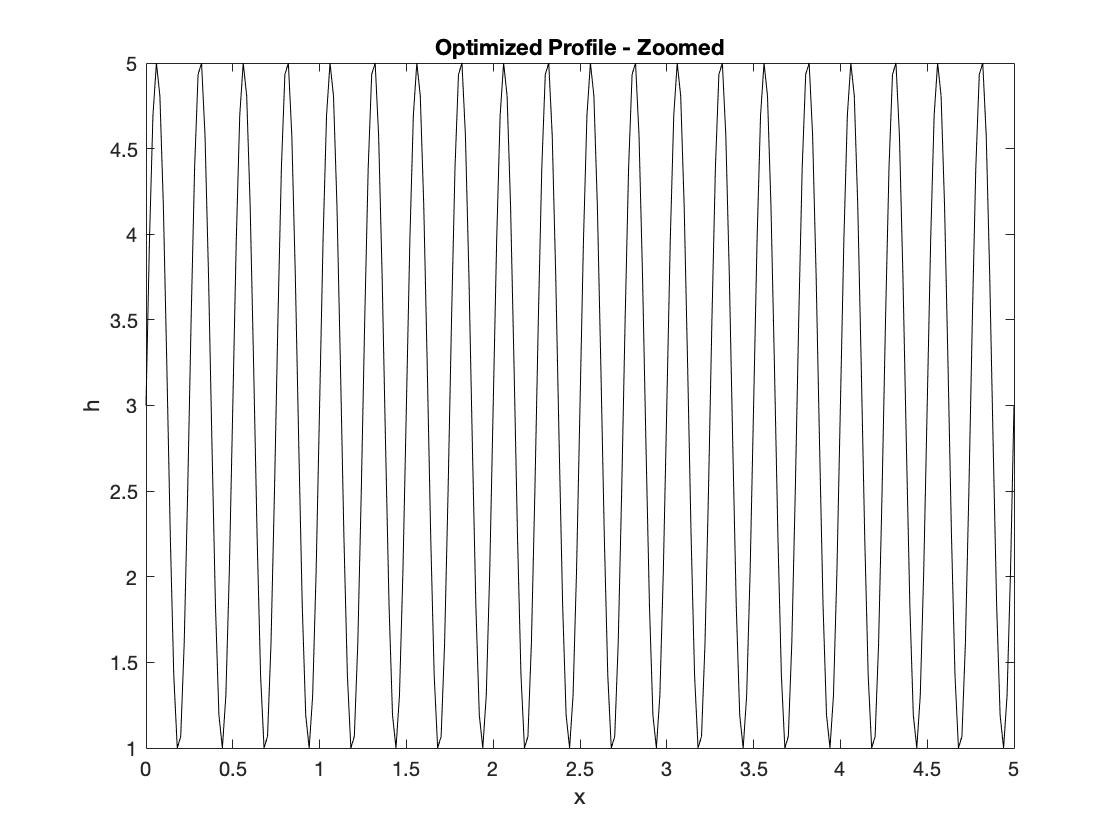
\includegraphics[width=\textwidth]{Mtd1_SP4_2}
         			\caption{Final Zoomed - Sinusoidal}
         			\label{fig: sin final zoomed}
         		\end{subfigure}
         		\caption{Optimized Profile using Sinusoidal Parameterization}
			\end{figure}
			\item Flux through Optimized profile: $58064.3129 \frac{W}{m^2}$
			\item Optimizer convergence:
			\begin{enumerate}
				\item Total number of iterations: $10$
				\item The total number of function calls: $242$
				\item Algorithm used: $Interior-Point$
				\begin{figure}[H]
					\centering
					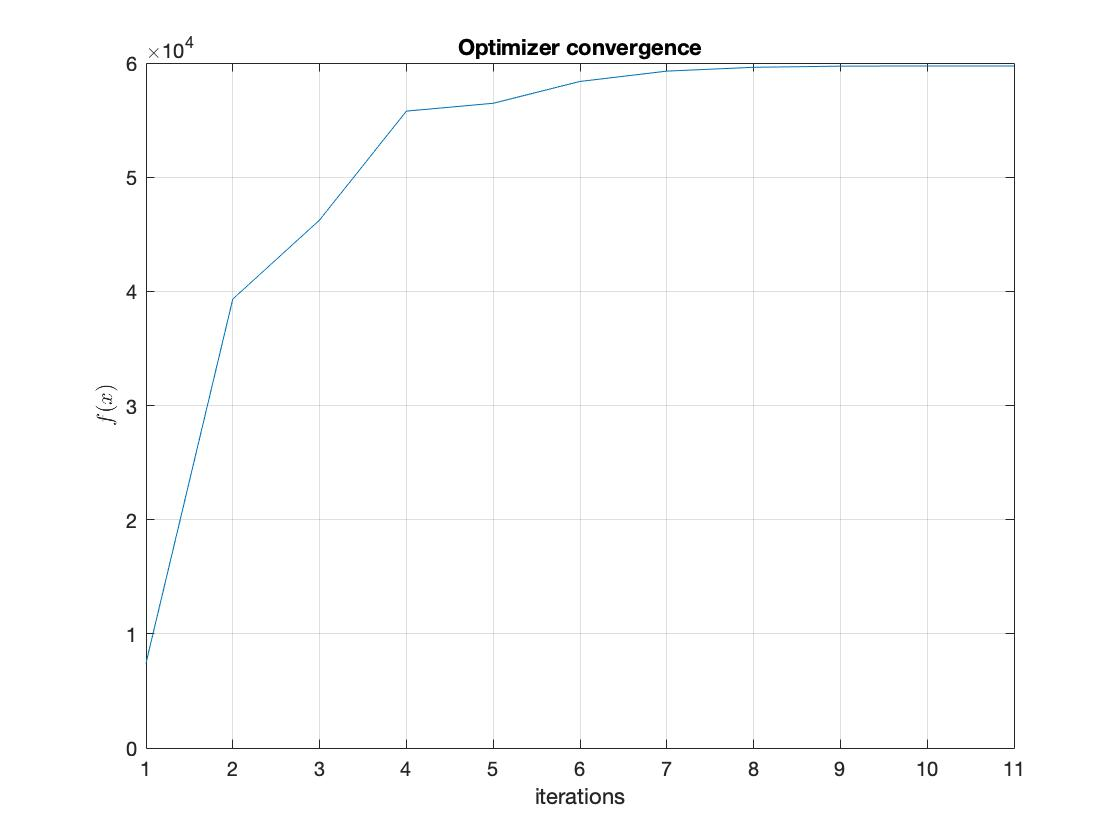
\includegraphics[width=0.5\textwidth]{Mtd1_SP4_3}
					\caption{Flux v Iteration - Sinusoidal}
					\label{fig: sin fluxIter} 
				\end{figure}
			\end{enumerate}
		\end{itemize}
	\item Triangular Parameterization
		\begin{itemize}
			\item Initial Condition : $a_0 = [3;2;10] \; \; \; a\in \mathbb{R}^{3}$
			\item Optimal Design Variable : \hyperlink{X-tri}{Found in Appendix}
			\item Final Top Profile: 
			\begin{figure}[H]
				\centering
				\begin{subfigure}[b]{0.45\textwidth}
         			\centering
         			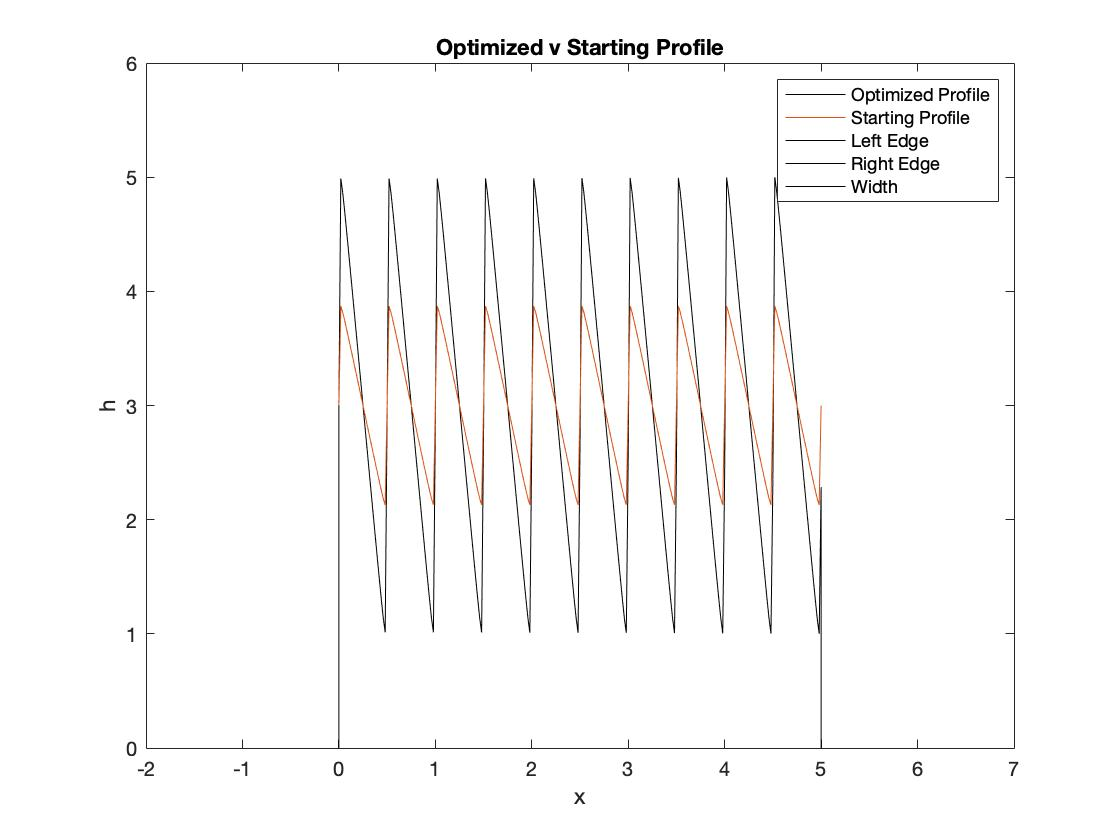
\includegraphics[width=\textwidth]{Mtd3_SP1_1}
         			\caption{Starting v Final - Triangular}
         			\label{fig: tri start v end}
         		\end{subfigure}
         		\hfill
			\begin{subfigure}[b]{0.45\textwidth}
         			\centering
         			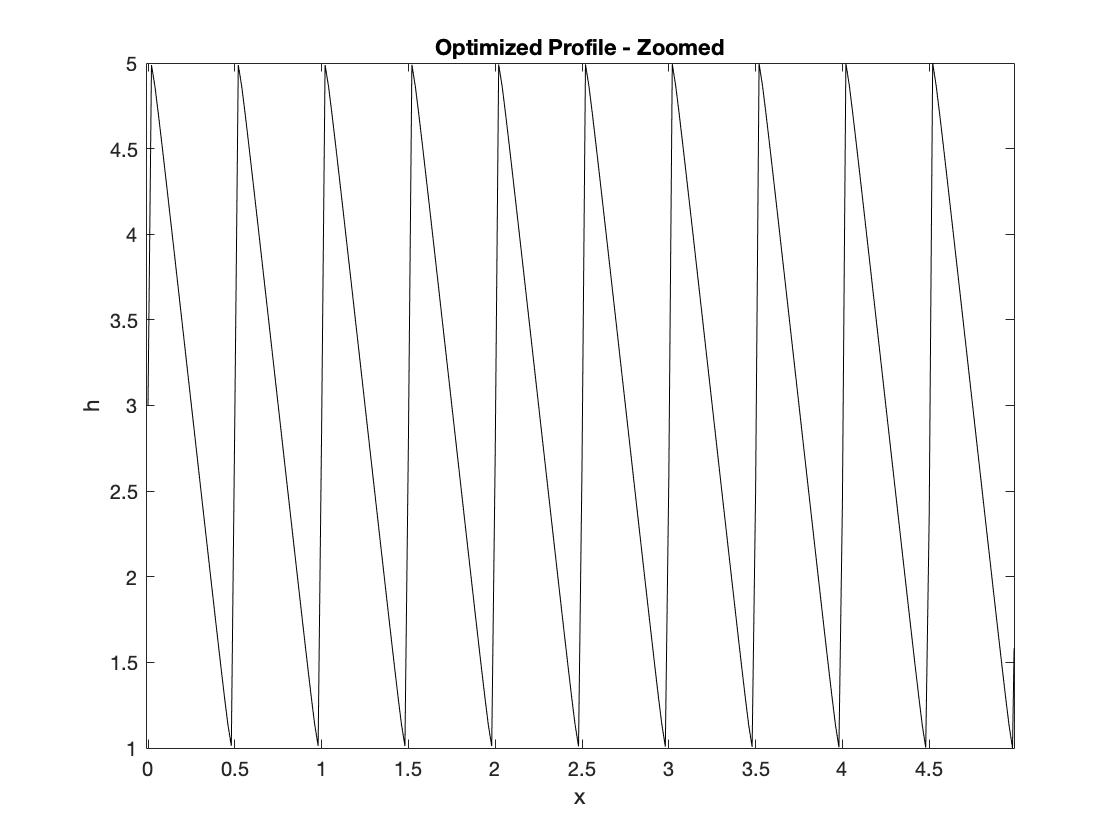
\includegraphics[width=\textwidth]{Mtd3_SP1_2}
         			\caption{Final Zoomed - Triangular}
         			\label{fig: tri final zoomed}
         		\end{subfigure}
         		\caption{Optimized Profile using Triangular Parameterization}
			\end{figure}
			\item Flux through Optimized profile: $40849.37706 \frac{W}{m^2}$
			\item Optimizer convergence:
			\begin{enumerate}
				\item Total number of iterations: $33$
				\item The total number of function calls: $138$
				\item Algorithm used: $Interior-Point$
				\begin{figure}[H]
					\centering
					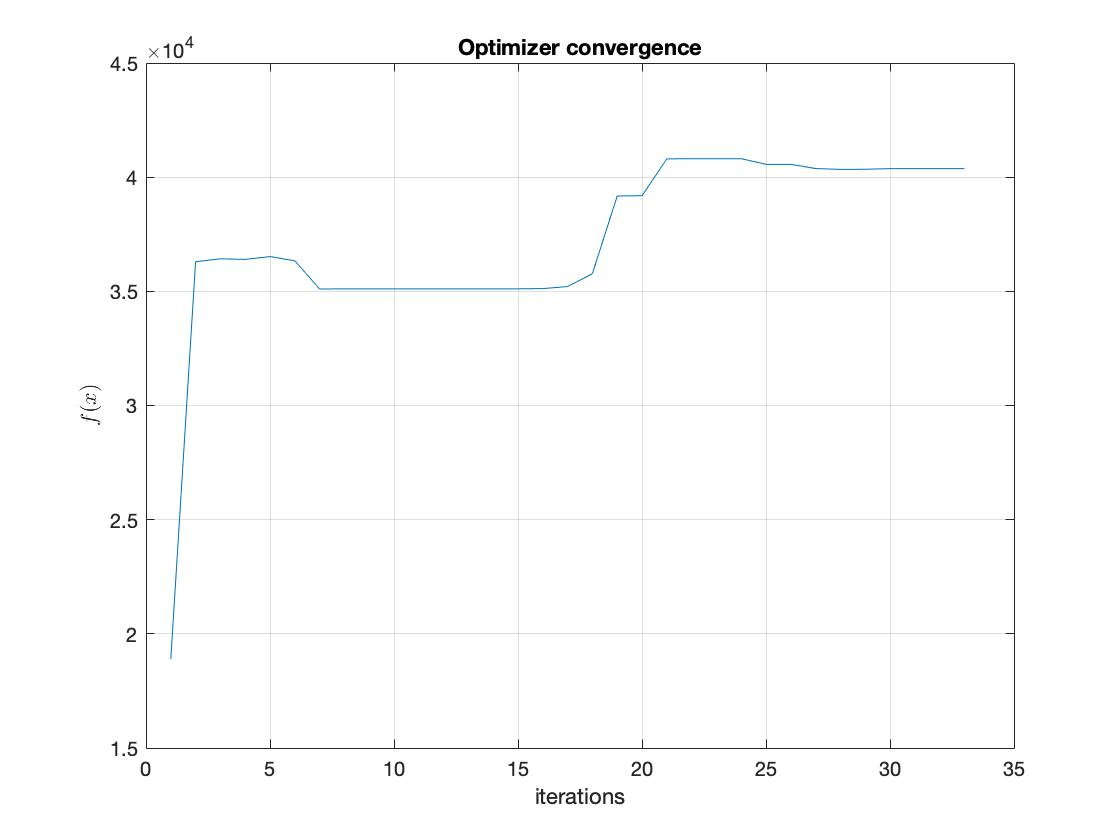
\includegraphics[width=0.5\textwidth]{Mtd3_SP1_3}
					\caption{Flux v Iteration - Triangular}
					\label{fig: tri fluxIter}
				\end{figure}
			\end{enumerate}
		\end{itemize}			
\end{enumerate}
Between the three methods and starting points, it is clear that the linear parameterization does not lead to the maximum flux that can possibly be obtained from the conditions and criteria specified because it leads to a profile which is a flat rectangle of dimensions $1cm$ x $5cm$ . The maximum flux that can come out of this profile can be analytically calculated and that is $7000 \frac{W}{m^2}$. The optimizer led to achieving a profile that can lead to a flux value of $6953.64 \frac{W}{m^2}$. \\
Both the sinusoidal and triangular parameterization leads to a significantly large flux compared to the result a linear parameterization produced (approximately 700\% and 500\% respectively). It is also observed that as the number of dimensions are increased for the sinusoidal parameterization, the heat flux value keeps increasing. The same phenomenon is observed if the frequency parameter of the triangular parameterization is increased and that leads to more saw tooth profiles. $N_x = N_y = 100$ is used for this study and Figure.\ref{fig:FluxVDim} shows this phenomena. 
\begin{figure}[h]
\centering
\begin{subfigure}[b]{0.45\textwidth}
\centering
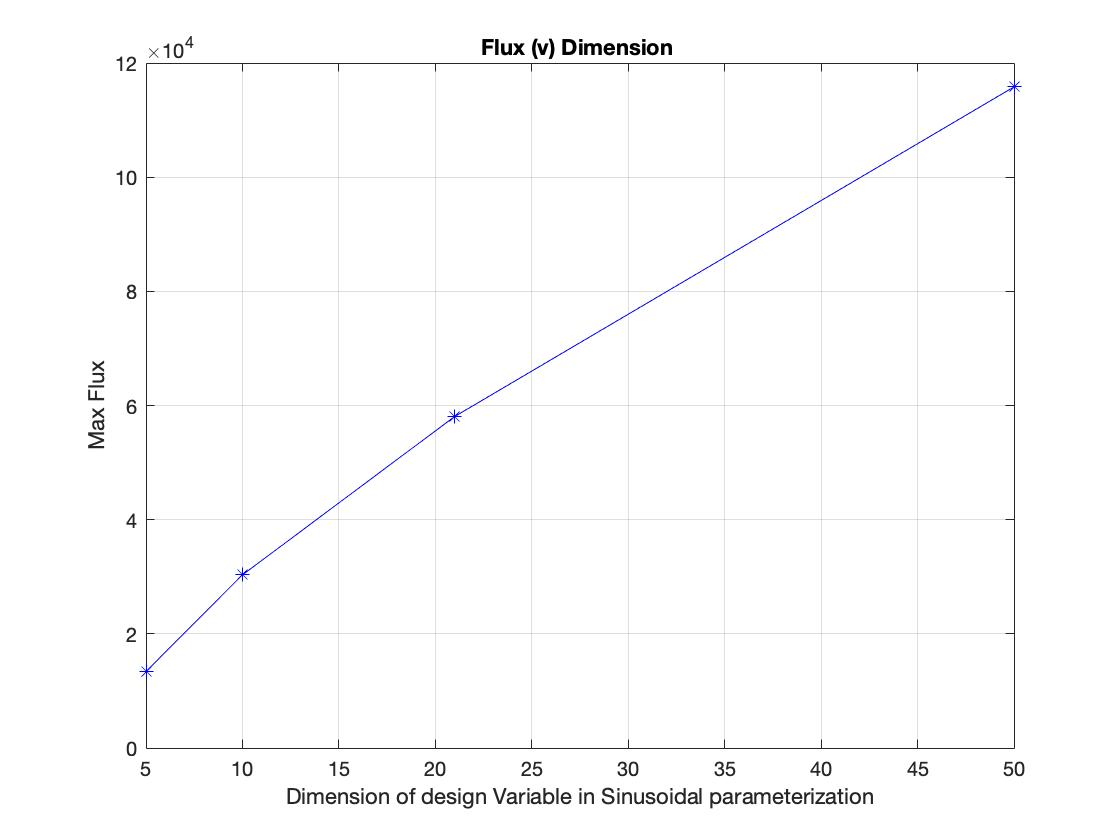
\includegraphics[width = \textwidth]{Flux_v_Dim}
\caption{Flux v Dimension of $a$ - Sinusoidal parameterization}
\end{subfigure}
\hfill
\begin{subfigure}[b]{0.45\textwidth}
\centering
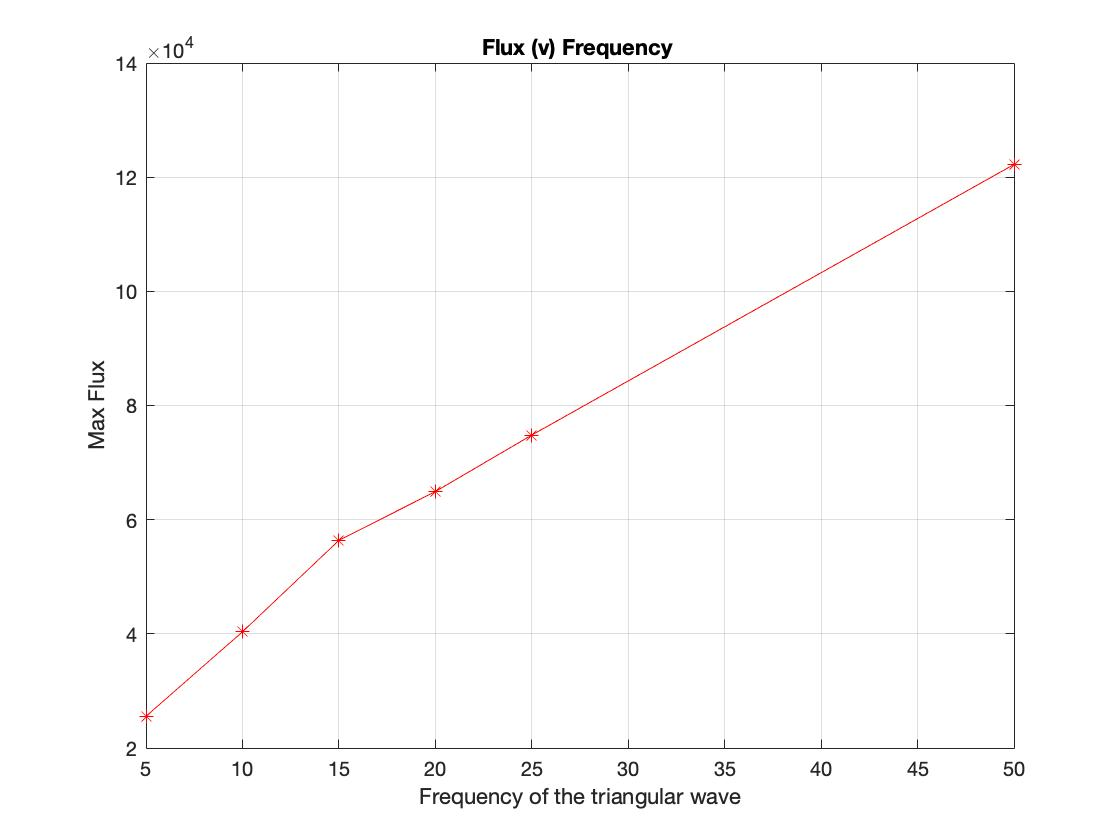
\includegraphics[width = \textwidth]{Flux_v_Freq}
\caption{Flux v $\nu$ of $a$ - Triangular parameterization}
\end{subfigure}
\caption{Increase of flux with certain aspects of design variable $a$}
\label{fig:FluxVDim}
\end{figure}
\section{Convergence Study}
The choice of $N_x = N_y = 100$ was entirely arbitrary and that leads to a decent approximation of what the heat flux would be for the optimized profile. But in order to find out what the closest possible to exact heat flux is through the optimized profile, refinement of mesh to have smaller finite volumes is necessary. Hence a convergence study will help figure out the relationship between a chosen optimized profile and the relationship with the size of the finite volumes. \\
Fig. \ref{fig: 25nu starting point} had an optimized design with a frequency of $\nu = 25$ using triangular parameterization. Fig.\ref{fig: 12 dim sin} has a starting point $a_0 \in \mathbb{R}^{12}$ and lastly, the third profile was of sinusoidal parameterization in Fig.\ref{fig: 10 dim sin} but with a starting point $a_0(1) = 3; a_0(2:10) = 0 $ and $a \in \mathbb{R}^{10}$. The intention for this design is two fold. One is to perform the convergence analysis and the other is to show how the choice of the starting point gives an optimal point belonging to different local minima. \\
Fig.\ref{fig: convergence analysis} shows how with finer and finer meshes, the results for Heat Flux converged to the closest approximation of the actual analytical solution. The problem that comes with finer meshes is the computational cost that comes with it. The same could be said about the increase in dimensionality in the case of a sinusoidal parameterization of the top profile. The biggest advantage of using a triangular parameterization was the fact that even with just 3 dimensions, it enables the optimizer to converge to results that can possibly produce high heat flux values. 
\begin{figure}[h]
\centering
\begin{subfigure}[b]{0.45\textwidth}
\centering
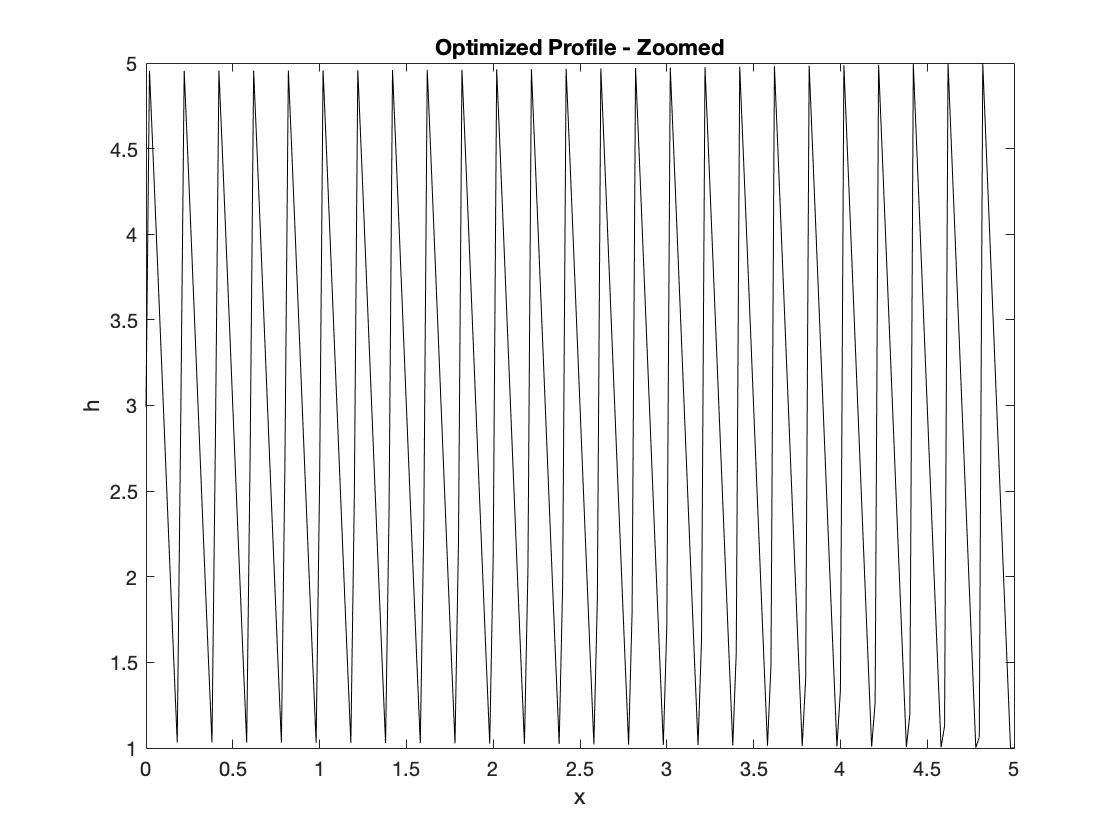
\includegraphics[width = \textwidth]{OptZoomed_Freq25}
\caption{Optimized Profile with $\Delta$ Parameterization $\nu = 25$}
\label{fig: 25nu starting point}
\end{subfigure}
\hfill
\begin{subfigure}[b]{0.45\textwidth}
\centering
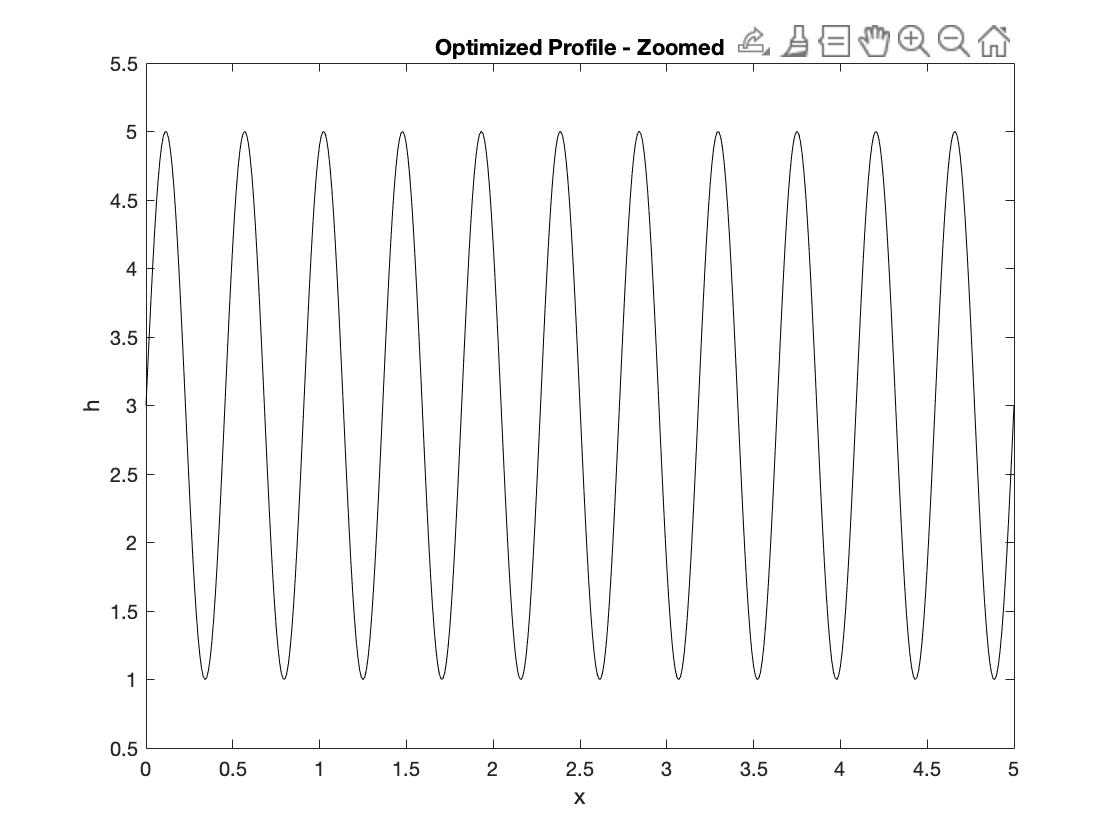
\includegraphics[width = \textwidth]{opt_zoomed_pt1_tri}
\caption{Optimized Profile with Sin Parameterization $a\in \mathbb{R}^{12}$}
\label{fig: 12 dim sin}
\end{subfigure}
\begin{subfigure}[b]{0.45\textwidth}
\centering
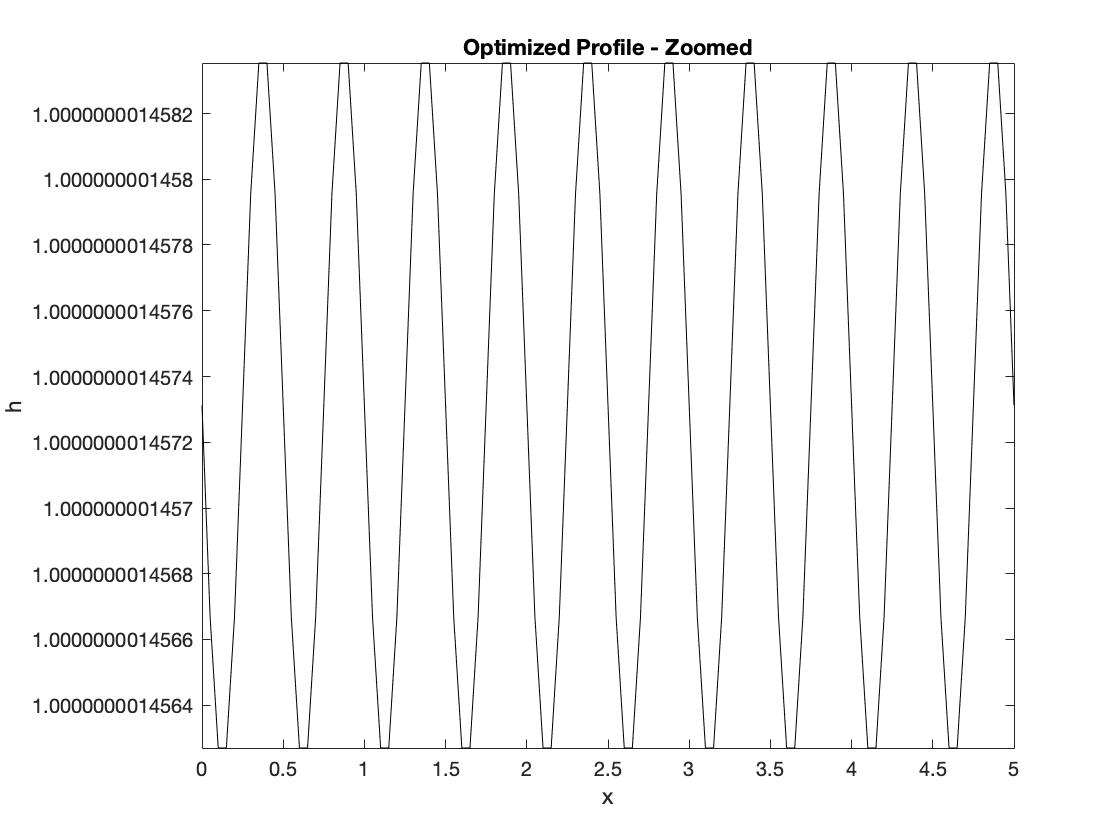
\includegraphics[width = \textwidth]{opt_zoomed_pt2}
\caption{Optimized Profile for a flat sin parameterization $a \in \mathbb{R}^{10}$}
\label{fig: 10 dim sin}
\end{subfigure}
\hfill
\begin{subfigure}[b]{0.45\textwidth}
\centering
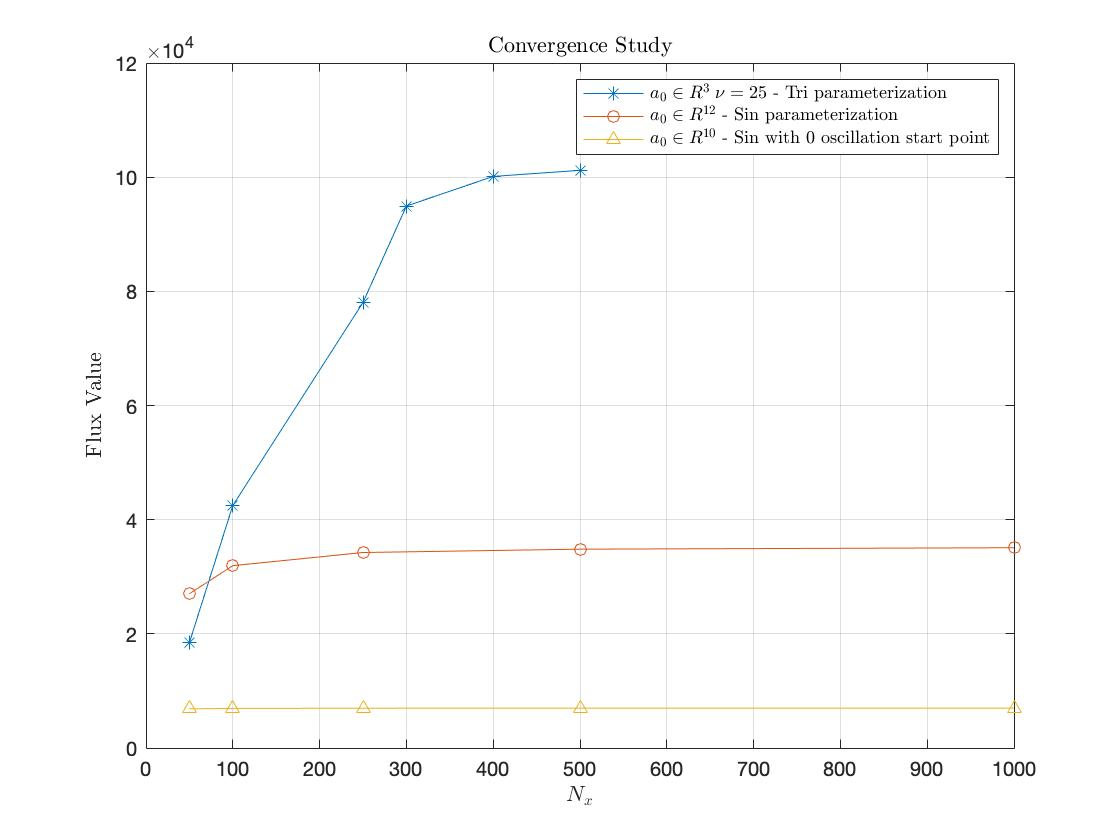
\includegraphics[width = \textwidth]{Convergence_study_2}
\caption{Convergence Analysis}
\label{fig: convergence analysis} 
\end{subfigure}
\caption{Convergence of Final Flux value with increasing mesh refinement}
\end{figure}

\section{Results and Inferences}
\begin{enumerate}
\item This project sheds light on the well known fact that in order to maximize heat transfer or heat flux from one medium to another, the most optimal design is to have structures called \textbf{Fins}. These are structures with very less thickness in order to increase the surface area of heat transfer. Both sinusoidal and triangular parameterization leads to creation of a \textbf{fin-like profile}. 
\item From a design stand point, it can be shown that different starting points or initial points lead to different optimal designs that satisfy the constraints or bounds. 
\item Another side note is that the number of iterations and function calls increase heavily if the initial point is out of the tolerable bounds. For example, an initial point with $a_0(1)=3; a_0(2:21)=0.5; a_0 \in \mathbb{R}^{21}$ gives a profile that is out of bounds as shown in Fig.\ref{fig: out of bounds}. The number of function calls were $1344$ and the maximum number of iterations was restricted to $60$. The Final Flux attained was $53111.309266 \frac{W}{m^2}$.Comparing this with the solution for a problem with the same dimensionality like in Fig.\ref{fig: linear start v end}, the clear increase in number of function calls and iterations can be seen. 
\begin{figure}[H]
\centering
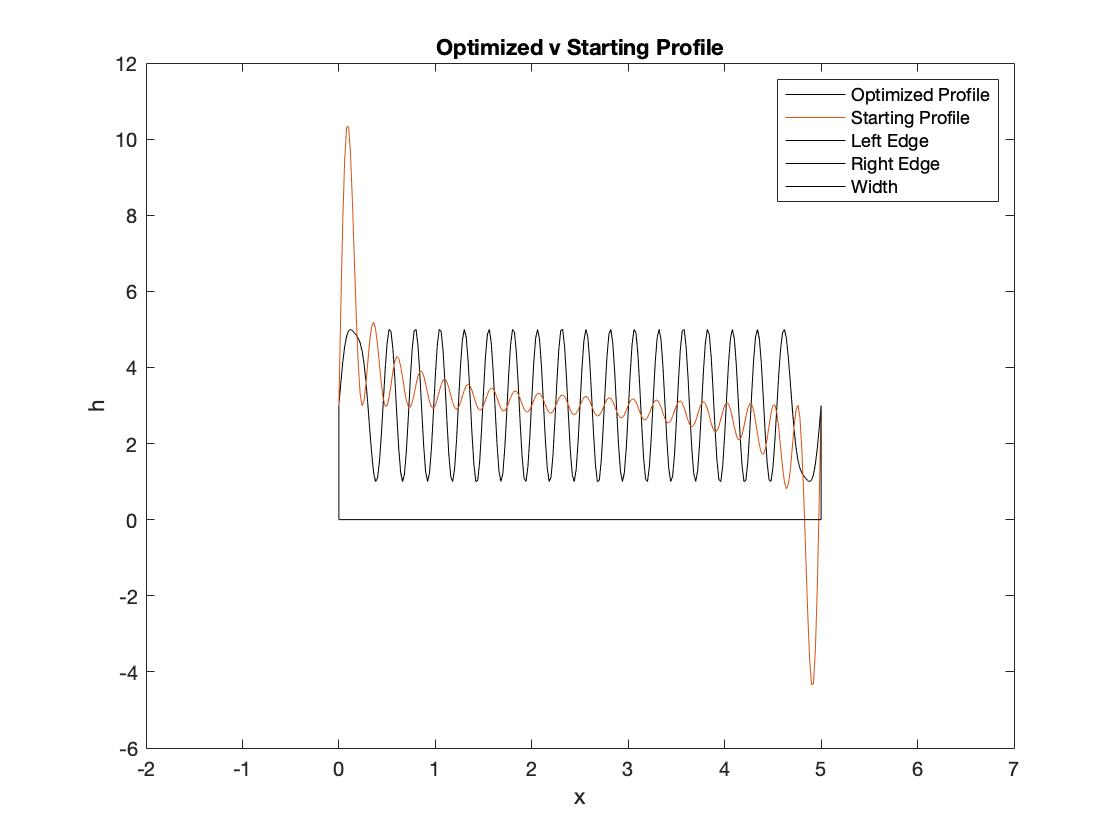
\includegraphics[width =0.5\textwidth]{infeasible_sp}
\caption{Optimal Profile if starting with an infeasible point}
\label{fig: out of bounds}
\end{figure}
\item Fig. \ref{fig:FluxVDim} is another clear indication that with more number of fins, the maximum heat flux will increase. That was evident with the rise in heat flux values with the increase in the number of dimensions of the design variable in the sinusoidal case and with the increase of frequency parameter in the triangular parameterization case.
\item From this project, the final flux values being reported are the following: \\
\begin{itemize}
\item Linear Parameterization of $a \in \mathbb{R}^{21}$ yields - $6993.64 \frac{W}{m^2}$ with $N_x = N_y = 1000$
\item Sinusoidal Parameterization of $a \in \mathbb{R}^{21}$ yields - $59741.29 \frac{W}{m^2}$ with $N_x = N_y = 500$
\item Triangular Parameterization of $a \in \mathbb{R}^3$ and with $\nu_0 = 25$ yields - $101299.8736 \frac{W}{m^2}$ with $N_x = N_y = 500$
\end{itemize}
\end{enumerate}
\newpage
\section{Appendix}

\begin{appendix}

\subsection{Optimal points from Optimizer:}
\hypertarget{X_linear}{X_{linear}} = \\$[1.00000000596375;-0.00211736922847506;-0.00211736921230914;-0.00214675654158376;... \\
-0.00214675654158372;-0.00103336585774427;0.00372561891272210;-0.00104535054108106;...\\
0.00250995878394754;-0.00191602678535082;0.00269913312708719;-0.00116146051702897;...\\
-0.00373671543331022;-0.00370640515815103;-0.00174780407094227;0.00508637365704515;...\\
0.00474105248772209;0.00172282541372274;-0.00305458551853304;0.00329743748706565;...\\
0.00214756553680345]
$ \\
\hypertarget{X-sin}{X_{sinusoidal}} = \\
$[2.99999996885313;-9.41854650580605e-10;1.01625785627599e-10;1.72461166932447e-09;...\\
2.13650671495380e-09;1.38715769824086e-09;-2.92563268723410e-10;-2.35288492567810e-09;...\\
-3.03543755880989e-09;-9.36670529000131e-10;-0.0218389278795468;3.79154438677764e-10;...\\
1.13461569109465e-09;-8.39196431264226e-10;-1.20349378889991e-09;-3.81241874638362e-11;...\\
1.94669430010950e-09;3.97997270171530e-09;4.32586722307759e-09;-1.84413351597820e-09;...\\
2.01893364029489]
$ \\
\hypertarget{X-tri}{X_triangular} = $[3.00062733283020;4.56749698436269;9.99841012519896]$

\subsection{Optimizer convergence - Flux value V Iterations}
Linear Parameterization Fig.\ref{fig: lin fluxIter} Flux value v Iterations: \\
\begin{table}[H]
\centering
\begin{tabular}{|c|c|}
\hline
Iteration & Flux Value \\
\hline
1 & 2.392837e+03 \\
2 & 4.980509e+03 \\
3 & 5.016815e+03 \\
4 & 6.759283e+03 \\
5 & 6.764436e+03 \\
6 & 6.764331e+03 \\
7 & 6.772434e+03 \\
8 & 6.774177e+03 \\
9 & 6.774173e+03 \\
10 & 6.774193e+03 \\
11 & 6.774193e+03 \\
12 & 6.774193e+03 \\
13 & 6.774194e+03 \\
\hline
\end{tabular}
\caption{Flux v Iterations - Linear parameterization}
\end{table}

Sinusoidal Parameterization Fig.\ref{fig: sin fluxIter} Flux value v Iterations: \\
\begin{table}[H]
\centering
\begin{tabular}{|c|c|}
\hline
Iteration & Flux Value \\
\hline
1 & 7.436319e+03 \\
2 & 3.932569e+04 \\
3 & 4.624590e+04 \\
4 & 5.578685e+04 \\
5 & 5.647216e+04 \\
6 & 5.838431e+04 \\
7 & 5.928845e+04 \\
8 & 5.962379e+04 \\
9 & 5.972434e+04 \\
10 & 5.974116e+04 \\
11 & 5.974129e+04 \\
\hline
\end{tabular}
\caption{Flux v Iterations - Sinusoidal parameterization}
\end{table} 

Triangular Parameterization Fig.\ref{fig: tri fluxIter} Flux value v Iterations: \\
\begin{table}[h]
\centering
\begin{tabular}{|c|c|}
\hline
Iteration & Flux Value \\
\hline
1 & 1.889699e+04 \\
2 & 3.629552e+04 \\
3 & 3.642467e+04 \\
4 & 3.639738e+04 \\
5 & 3.652243e+04\\
6 & 3.633551e+04\\
7 & 3.510292e+04\\
8 & 3.510715e+04\\
9 & 3.510792e+04\\
10 & 3.510791e+04\\
11 & 3.510792e+04\\
12 & 3.510793e+04\\
13 & 3.510800e+04\\
14 & 3.510833e+04\\
15 & 3.511008e+04\\
16 & 3.512022e+04\\
17 & 3.520962e+04\\
18 & 3.577353e+04\\
19 & 3.917566e+04\\
20 & 3.918646e+04\\
21 & 4.080098e+04\\
22 & 4.080920e+04\\
23 & 4.080888e+04\\
24 & 4.080932e+04\\
25 & 4.056148e+04\\
26 & 4.056181e+04\\
27 & 4.037784e+04\\
28 & 4.033888e+04\\
29 & 4.034618e+04\\
30 & 4.037414e+04 \\
31 & 4.037414e+04 \\
32 & 4.037414e+04 \\
33 & 4.037414e+04\\
\hline
\end{tabular}
\caption{Flux v Iterations - Triangular parameterization}
\end{table}

\subsection{Convergence Analysis}
Triangular Parameterization Optimized profile with frequency 25:\\ 
\begin{table}[H]
\centering
\begin{tabular}{|c|c|}
\hline
$N_x$ & Flux Value \\
\hline
$50$ & $1.844683713076328e+04$\\
$100$ & $4.248849784574824e+04$ \\
$250$ & $7.805146638013054e+04$\\
$300$ & $9.494107046818522e+04$\\ 
$400$ & $1.001292884539378e+05$\\
$500$ & $1.012998736898211e+05$\\
\hline
\end{tabular}
\caption{$N_x$ v Flux - Case 1}
\end{table} 

Sinusoidal parameterization with $a \in \mathbb{R}^{12}$: \\
\begin{table}[H]
\centering
\begin{tabular}{|c|c|}
\hline
$N_x$ & Flux Value \\
\hline
$50$ & $2.702959713192348e+04$\\
$100$ & $3.194138632807931e+04$ \\
$250$ & $3.424638727249664e+04$\\
$500$ & $3.483118953557032e+04$\\ 
$1000$ & $3.508359374896967e+04$\\
\hline
\end{tabular} 
\caption{$N_x$ v Flux - Case 2}
\end{table} 

Sinusoidal Parameterization with $ a_0 \in \mathbb{R}^{12}; \; \; a_0(1) = 3; a_0(2:end) = 0;$ \\ 
\begin{table}[H]
\centering
\begin{tabular}{|c|c|}
\hline
$N_x$ & Flux Value \\
\hline
$50$ & $6.865384605379591e+03$\\
$100$ & $6.931372538918941e+03$ \\
$250$ & $6.972222212062424e+03$\\
$500$ & $6.986055766722282e+03$\\ 
$1000$ & $6.993013961830300e+03$\\
\hline
\end{tabular} 
\caption{$N_x$ v Flux - Case 3}
\end{table}
\subsection{MATLAB Code}
The $MATLAB$ code that was created to perform this analysis has been attached as a part of the appendix for all three methodologies. 
\end{appendix}
\end{document}